\begin{figure}
    \begin{subfigure}[c]{0.25\textwidth}
        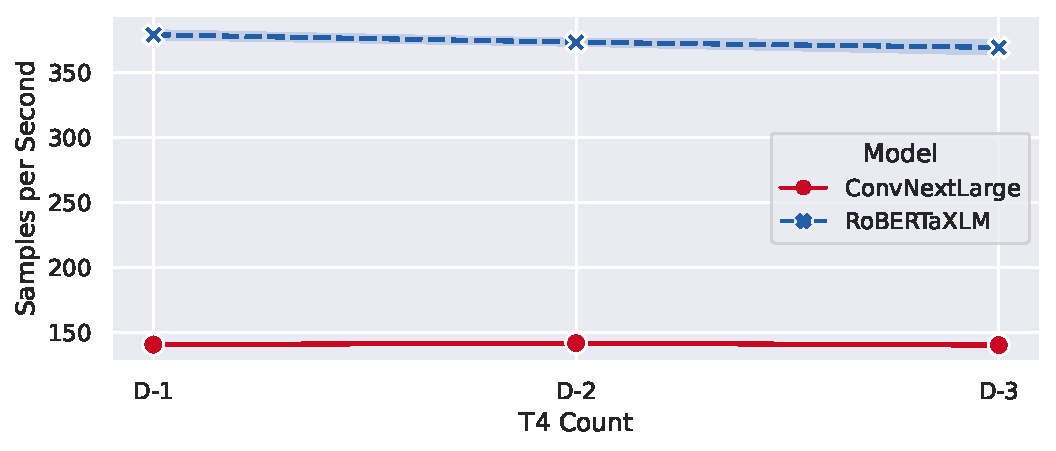
\includegraphics[width=\textwidth]{figures/misc/multi-cloud-performance}
        \vspace{-15pt}
        \caption{Throughput}
        \label{fig:multi-cloud-throughput}
    \end{subfigure}
    \begin{subfigure}[c]{0.22\textwidth}
        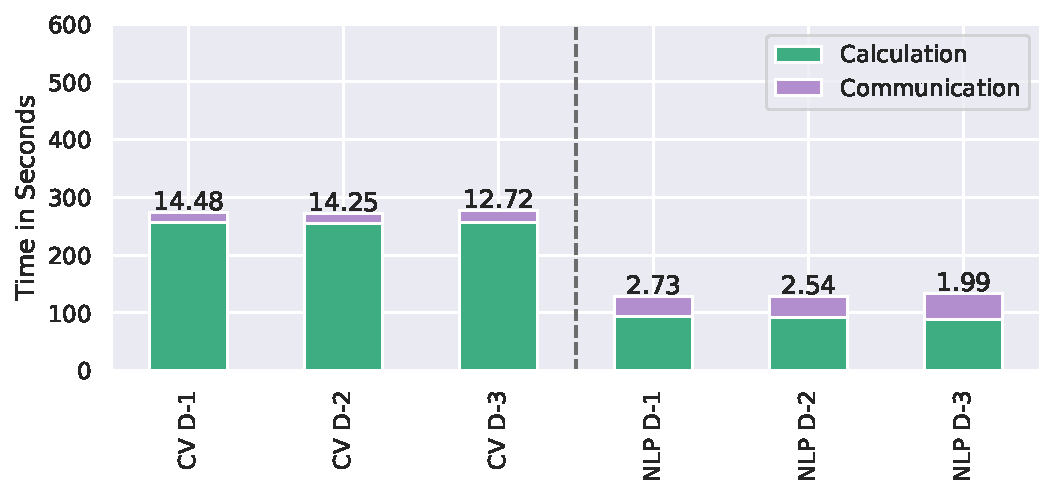
\includegraphics[width=\textwidth]{figures/misc/multi-cloud-performance-granularity}  
        \vspace{-15pt}
        \caption{Granularity}
        \label{fig:multi-cloud-granularity}
    \end{subfigure}
    \vspace{-10pt}
    \caption{Multi-cloud performance for CV and NLP.}
    \label{fig:multi-cloud-performance}
    \vspace*{-5mm}
\end{figure}

Using multiple cloud providers makes sense if we want to use resources cost-effectively and have additional reliability.
In our scenario, we are interested in what throughput per \$ can be expected and if any barriers prevent multi-cloud training.
However, one can also consider the data center's carbon footprint, which can change depending on the season and time of day.
Carbon-aware DL training could select spot instances from data centers based on current carbon emissions\footnote{https://cloud.withgoogle.com/region-picker/}.
\vspace*{-2mm}
\begin{table}[h]
    \scalebox{0.75}{
    \begin{subtable}[h]{0.30\textwidth}
        \centering
        \begin{tabular}{l|rrr}
        \backslashbox{\textbf{From}}{\textbf{To}}     & \textbf{GC} & \textbf{AWS} & \textbf{Azure} \\ \hline
        \textbf{GC}    & \cellcolor[HTML]{67F13A}6.35 & \cellcolor[HTML]{b2f13a}1.52 & \cellcolor[HTML]{fadc24}0.45 \\
        \textbf{AWS}   & \cellcolor[HTML]{b2f13a}1.81 & \cellcolor[HTML]{67F13A}4.87 & \\
        \textbf{Azure} & \cellcolor[HTML]{fadc24}0.47 & & \cellcolor[HTML]{67F13A}7.63
        \end{tabular}
        \caption{Single stream TCP throughput in Gbits.}
        \label{tab:multicloud-bandwidth}
    \end{subtable}
    }
    \scalebox{0.75}{
    \begin{subtable}[h]{0.30\textwidth}
        \centering
        \begin{tabular}{l|rrr}
        \backslashbox{\textbf{From}}{\textbf{To}}     & \textbf{GC} & \textbf{AWS} & \textbf{Azure} \\ \hline
        \textbf{GC}    & \cellcolor[HTML]{67F13A}0.71  & \cellcolor[HTML]{b2f13a}15.3 & \cellcolor[HTML]{fadc24}51.22 \\
        \textbf{AWS}   & \cellcolor[HTML]{b2f13a}13.85 & \cellcolor[HTML]{67F13A}0.15 & \\
        \textbf{Azure} & \cellcolor[HTML]{fadc24}49.80 & & \cellcolor[HTML]{67F13A}1.56
        \end{tabular}
        \caption{ICMP Latency in ms.} 
        \label{tab:multicloud-ping}
    \end{subtable}
    }
    \caption{Average multi-cloud throughput and latency.}
    \label{table:multicloud-network-profile}
    \vspace*{-8mm}
\end{table}

We have compiled the current prices for spot and on-demand instances for T4 GPUs with 8 CPU cores and the egress costs for three well-known cloud providers, GC~\cite{gcweb}, AWS~\cite{awsweb}, and Azure~\cite{azureweb} (\Cref{tab:cloud-pricing}).
There are two different pricing concepts. 
On the one hand, there are GC and Azure, which offer relatively cheap instances, with 69\% and 73\% savings over on-demand pricing, respectively, and relatively expensive egress charges between continents of up to 0.15\$/GB.
On the other hand, there is AWS, where the spot instance is only 51\% cheaper than the on-demand instance and more than twice as expensive as GC or Azure. 
However, the egress fees here are much cheaper at only 0.02\$/GB.
Because of the additional offerings around compute, such as networking, identity and cost management, and tooling, it is not easy to fairly compare cloud providers. Therefore, we will limit ourselves to network and VM costs.

With the multi-cloud experiments from this section, we want to evaluate the following scenarios:
First, partially switching from one provider to another without stopping the training.
Second, scaling resources in the same region when one of the cloud providers is already at capacity for spot-priced VMs or the current price is too high~\cite{9975369}. We know from ~\Cref{sec:geodistributed-performance} that scaling resources in the same location can significantly improve performance, which may only be possible using additional cloud providers. 

\textbf{Experimental design}. To enable a fair comparison between the different cloud providers, we rented hardware as identically as possible in the same region.
We used each provider's default settings and only changed the hardware specifications.
For GC, it is the same instance as in ~\Cref{sec:geodistributed-performance}, the \texttt{n1-standard-8} in \texttt{us-west1}, with eight cores and 30 GB RAM. At AWS, it is a \texttt{gd4n.2xlarge} instance with eight cores and 32 GB in the \texttt{us-west-2c} region.
Unfortunately, we had to make two compromises with Azure.
There was only the combination of four cores and 30 GB RAM (\texttt{NC4as\_T4\_v3}), and there were no T4 GPU resources available in the \texttt{us-west}, so we had to fall back to \texttt{us-south-2}.
 
The network profiling between all cloud providers in ~\Cref{table:multicloud-network-profile} shows that their intra-cloud connectivity is comparably fast with 6.4, 4.9, and 7.6~Gbits for GC, AWS, and Azure, respectively.
All connections are mostly symmetric, with inter-cloud connectivity between GC and AWS providing up to 1.8~Gbits and a ping of 15.3ms, indicating that while they are likely not in the same data center, they are close to each other and connected to the same Internet exchange point.
However, connectivity to Azure could be better since it operates in a different zone, with a bandwidth of 0.5~Gbits and a ping of 51ms.

Our experimental setup consists of four GPUs with different contributions from each cloud provider. D-1 is the baseline with four GPUs at GC, D-2 with two GPUs each at GC and AWS, and D-3 with two GPUs at GC and Azure.
We compare the impact of moving two of the four VMs to a different cloud provider to see the impact on cost and throughput.

\textbf{(1) No inter-cloud throughput penalty}. ~\Cref{fig:multi-cloud-performance} shows the throughput and granularity of each multi-cloud experiment.
CV and NLP runs have essentially identical throughput regardless of the combination of cloud providers.
Only the D-3 experiments show a very slight slowdown in communication time, reflected in the lower granularity score (\Cref{fig:multi-cloud-granularity}) of 12.72 in CV and 1.99 in NLP compared to the D-1 baseline scores of 14.48 and 2.73, respectively.
Actual throughput was between 1-2\% slower than the baseline, which is negligible and only related to the slightly worse connection to the Azure data center.
These results confirm our observation from ~\Cref{sec:geodistributed-performance} that network connectivity determines scalability, and one can easily train in a multi-cloud scenario.
\vspace*{-2mm}

\begin{figure}[h]
    \begin{subfigure}[c]{0.48\textwidth}
        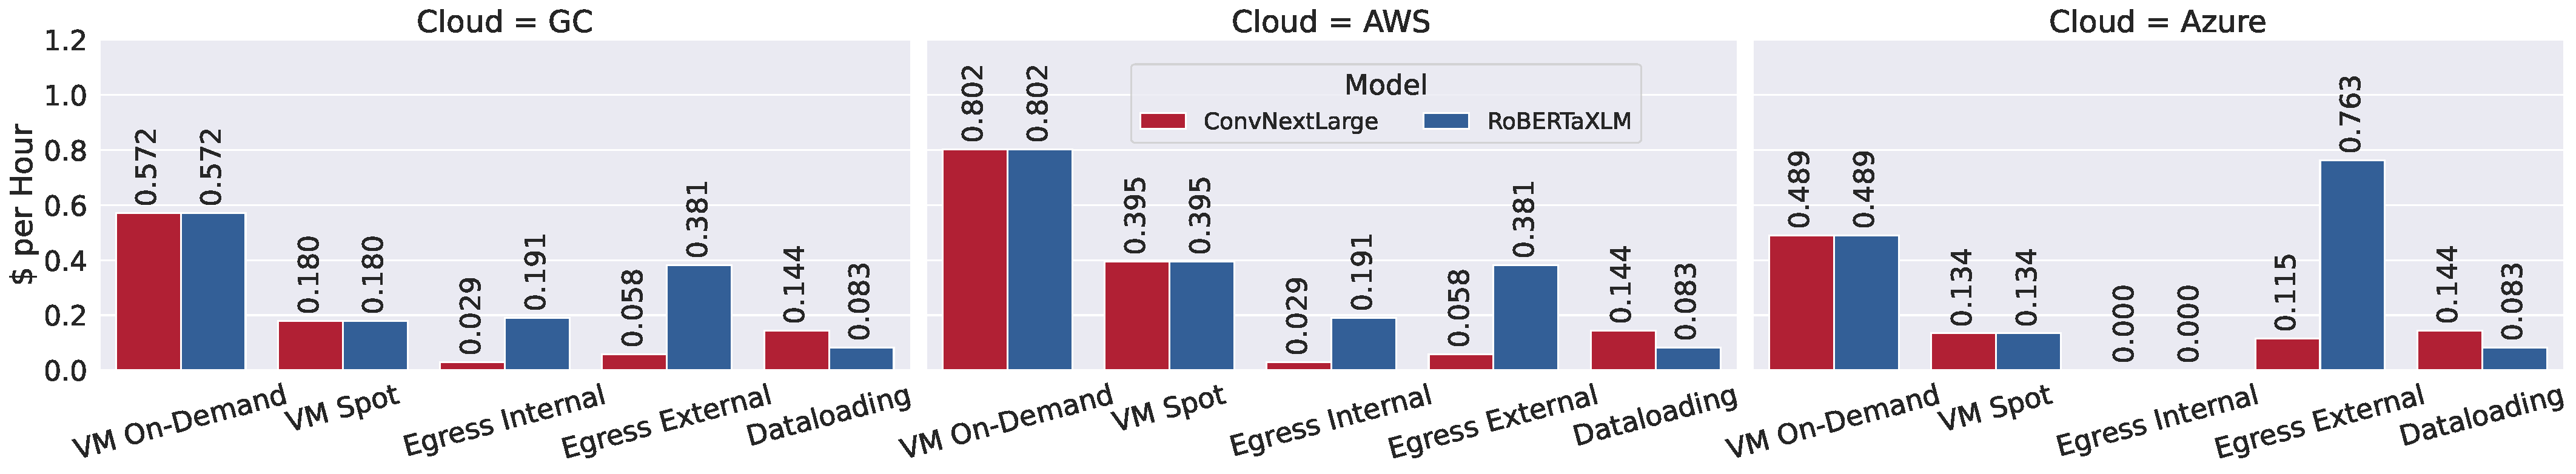
\includegraphics[width=\textwidth]{figures/misc/multi_cloud_cost_comparison_d3}
        \vspace{-15pt}
        \caption{Intra- and inter-zone in the US region (D-2/3).}
        \label{fig:multi-cloud-costs-d3}
    \end{subfigure}
    \begin{subfigure}[c]{0.48\textwidth}
        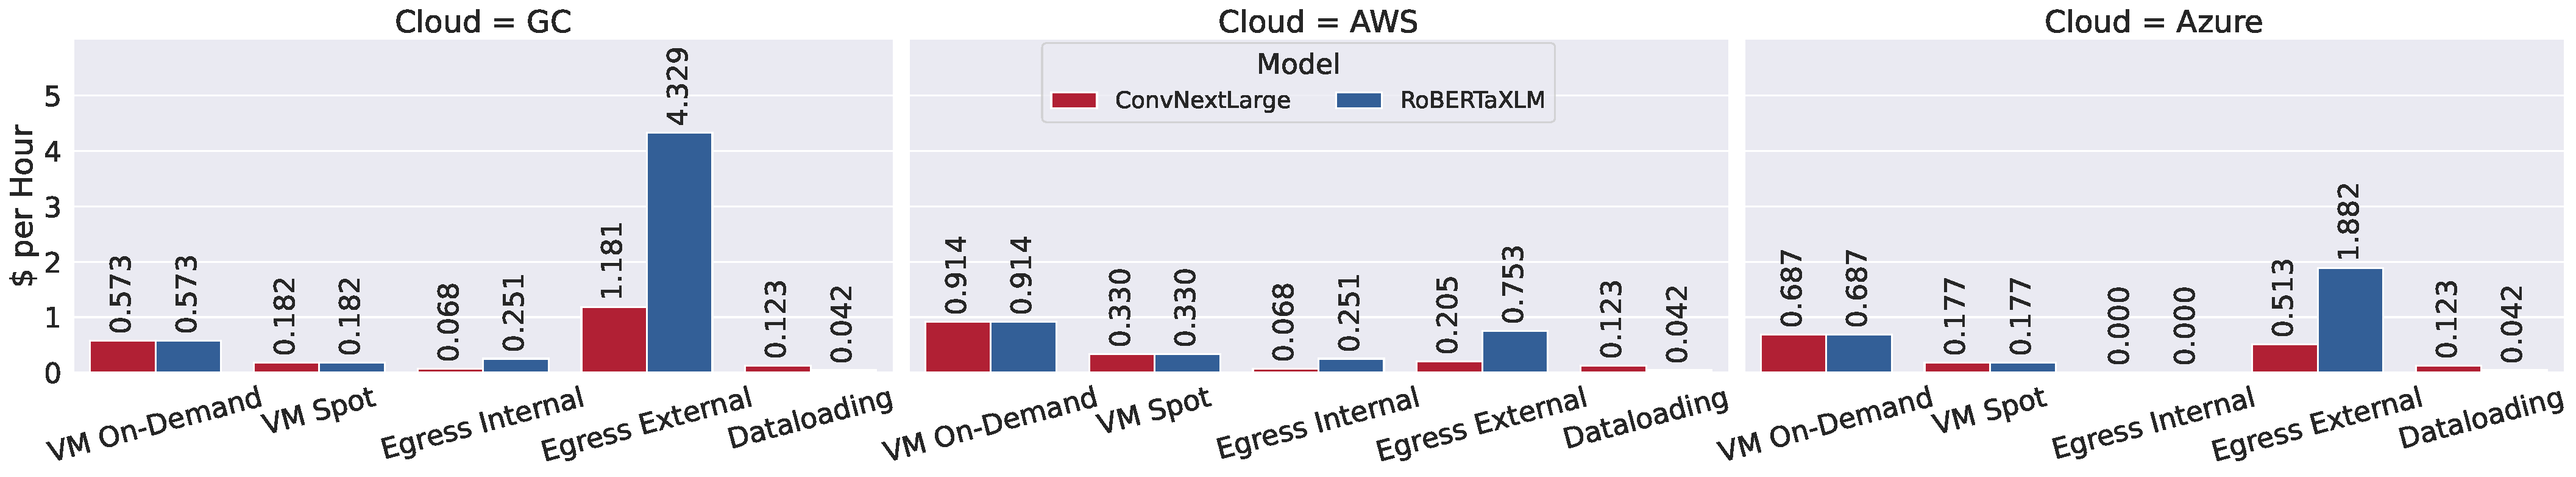
\includegraphics[width=\textwidth]{figures/misc/multi_cloud_cost_comparison_c8}  
        \vspace{-15pt}
        \caption{Intercontinental in the US, EU, ASIA and AUS (C-8).}
        \label{fig:multi-cloud-costs-c8}
    \end{subfigure} 
    \vspace{-10pt}
    \caption{Costs breakdown for the multi-cloud D-2/3 and intercontinental C-8 experiments.}  
    \label{fig:normalized-multi-cloud-costs}
    \vspace*{-5mm}
\end{figure}  
 
\textbf{(2) External egress costs can overshadow VM costs.} One drawback to training in multiple regions or zones is that egress traffic can incur additional costs depending on the cloud provider.
We have summarized the cost of egress traffic within a zone (intra-zone), between zones in each region (inter-zone), and between continents in ~\Cref{tab:cloud-pricing}. 
Notably, any traffic to Oceania (Australia, New Zealand, and others, abbreviated as OCE) generates the highest cost of 0.15\$/GB for GC.
We have broken down the costs for the multi-cloud experiment in ~\Cref{fig:multi-cloud-costs-d3} on an hourly per-VM basis. 
With only four peers in the D-1/2/3 experiments, we have an N-to-N communication, i.e., each peer sends its gradients to every other peer.
This means that $\frac{1}{3}$ of the egress was internal to the partner VM in the same cloud, and the remaining $\frac{2}{3}$ went to the remaining two peers in the other cloud.

First, loading data from Backblaze costs 0.01\$/GB from anywhere in the world, which gives us a rate of 0.144\$/h for the CV and 0.083\$/h for the NLP experiments.
Even when CV throughput is less than half of the NLP model (\Cref{fig:multi-cloud-throughput}), images are much larger than text, resulting in a higher data rate.
While this is close to the spot instance costs of GC (0.18\$/h) and Azure (0.134\$/h), these are one-time costs until the entire dataset is downloaded and retrieved from the disk cache, assuming local storage is large enough.
A more detailed comparison of cloud provider storage offerings is beyond our scope, but current prices range from 0.02\$/GB to 0.14\$/GB in various GC regions, making our setting (B2) competitive.
% GC: 0.381 / 0.18 = 2.1166
%>>> 0.180 + 0.191 + 0.381 + 0.083
%0.835
%>>> 0.395 + 0.191 + 0.381 + 0.083
%1.05
%>>> 0.131 + 0.763 + 0.083
%0.977
%>>> cv_gc_aws = 0.762 + 1.192
%>>> cv_gc_aws
%1.954
%>>> cv_gc_azure = 0.762 + 0.363
%>>> cv_gc_azure
%1.125
%>>> cv_gc_azure / cv_gc_aws
%0.5757420675537359
%>>> nlp_gc_aws = 0.180 + 0.191 + 0.381 + 0.083 + 0.395 + 0.191 + 0.381 + 0.083
%>>> nlp_gc_azure = 0.180 + 0.191 + 0.381 + 0.083 + 0.131 + 0.763 + 0.083
%>>> nlp_gc_azure / nlp_gc_aws
%0.9612732095490717

Second, the external egress costs for the NLP experiments are very high compared to the other costs.
They are 2.2x higher than the spot instance for GC and 5.7x higher for Azure, as the traffic costs in the US zone are 0.01\$/GB and 0.02\$/GB, respectively.
The Azure cost is even higher (0.763\$/h) than the on-demand instance price of 0.489\$/h.
The CV experiments are much less affected due to the smaller model size, but Azure still manages to almost match its spot instance price of 0.134\$/h with the external egress cost of 0.115\$/h.

Finally, the total compute cost, including egress and data loading in this multi-cloud constellation, is the sum of all the cloud providers' prices times the number of VMs used.
For the CV experiments, GC, AWS, and Azure cost 0.762\$/h, 1.192\$/h, and 0.363\$/h, respectively, making the combination of GC with Azure 42\% cheaper than GC with AWS.
For the NLP experiments, GC, AWS, and Azure cost 0.835\$/h, 1.05\$/h, and 0.973\$/h, respectively, and GC combined with Azure is better than GC with AWS by a smaller margin of 3.9\%.

However, the intercontinental network egress prices for both GC and Azure are up to 15 times higher than the inter-zone prices, so what about the cost-effectiveness compared to geo-distributed experiments?


\textbf{(3) Geo-distributed egress can incur most of the cost.} To illustrate the cost of intercontinental training, we use our C-8 experiment with two VMs in the US, EU, ASIA, and AUS from ~\Cref{sec:geodistributed-performance} to plug in the cost for each cloud provider.
The egress costs are calculated slightly differently than in the D-2 and D-3 experiments because four groups of two VMs average locally and then distribute the gradients across the other groups.
This results in $\frac{8}{20}$ internal egress calls (two calls between each group), $\frac{6}{20}$ intercontinental egress calls (two calls between three regions), and $\frac{6}{20}$ AUS egress calls (three regions share their gradients with AUS and vice versa).

~\Cref{fig:multi-cloud-costs-c8} shows the resulting egress traffic cost per VM.
The high cost between continents quickly scales to a multiple of the remaining cost for CV and NLP with GC and Azure.
For NLP, the external egress cost for GC is 4.329\$/h, more than 90\% of the total cost per VM (4.804\$/h).
Even if Azure has a more moderate rate of 0.02\$/GB for intercontinental communication and only 0.08\$/GB for OCE traffic, this still results in 1.882\$/h external egress cost (2.101\$/h total).
This is in contrast to AWS, which has a cap of 0.02\$/GB to any location, resulting in the best total cost of 1.376\$/h per VM.
The relatively high AWS instance cost compares favorably to the other cloud providers regarding geo-distributed training.
Keeping egress traffic in mind when deciding to scale to other continents is essential, as it can be the most significant part of the total cost.
This raises another question: If egress traffic matters so much, how does model size affect it?
% GC
%>>> 4.329 + 0.042 + 0.251 + 0.182
%4.804
%>>> 4.329 / 4.804
%0.9011240632805994

% Azure
%>>> 1.882 + 0.042 + 0.177
%2.101
%>>> 0.753 + 0.042 + 0.251 + 0.395
%1.441

% AWS
%>>> 0.753 + 0.251 + 0.042 + 0.330
%1.3760000000000001
\vspace*{-3mm}
\begin{figure}[h]
    \begin{subfigure}[c]{0.225\textwidth}
        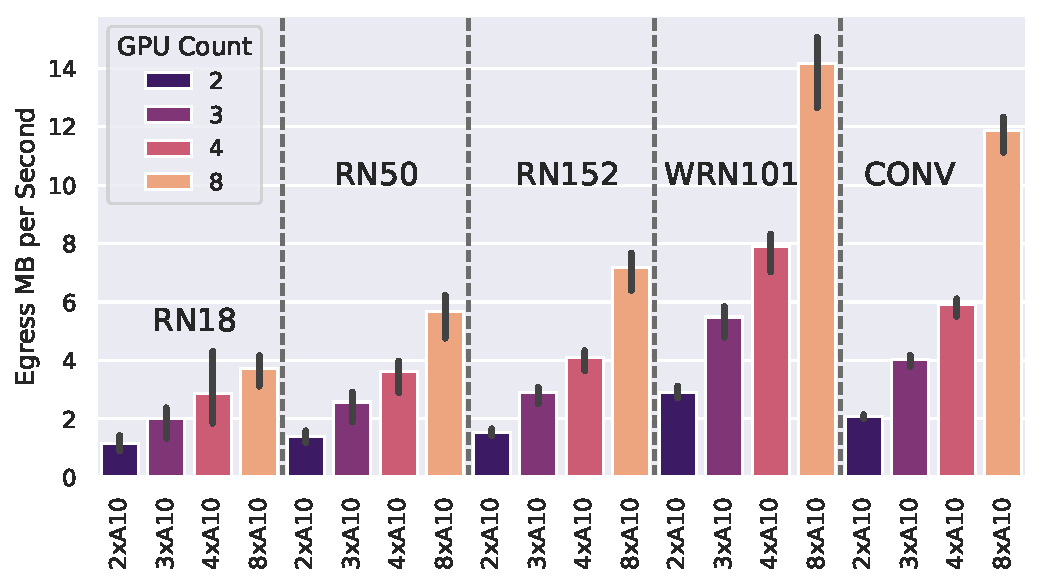
\includegraphics[width=\textwidth]{figures/misc/cv_baseline_egress}
        \vspace{-15pt}
        \caption{CV}
        \label{fig:cv-baseline-egress}
    \end{subfigure}
    \begin{subfigure}[c]{0.23\textwidth}
        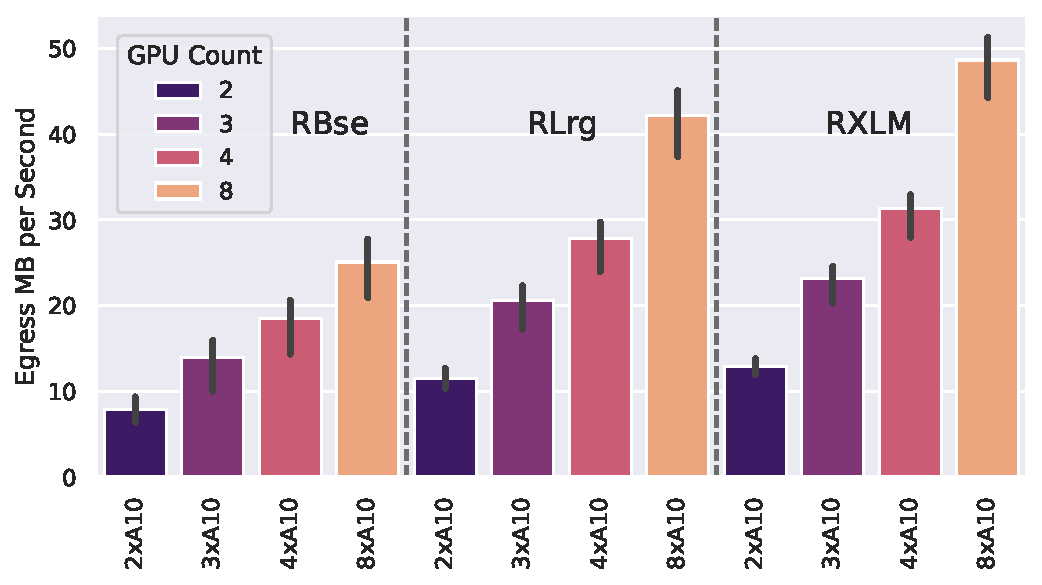
\includegraphics[width=\textwidth]{figures/misc/nlp_baseline_egress}  
        \vspace{-15pt} 
        \caption{NLP}
        \label{fig:nlp-baseline-egress} 
    \end{subfigure}
    \vspace{-10pt}
    \caption{Baseline egress rate on 2-8 A10 GPUs.}
    \label{fig:baseline-egress}
    \vspace*{-4mm} 
\end{figure} 
 
\textbf{(4) Small models have lower egress rates than larger models.} Model size affects two parts of the distributed training time.
First, the larger the model, the slower the averaging, and the higher the cost is due to the size of the gradients.
However, a large model will be averaged less frequently because the calculation time is much higher, which can result in a lower egress cost per hour.
To analyze this, we can review the experiments in ~\Cref{sec:model-suitability}, where we evaluate different model sizes with different numbers of GPUs.
~\Cref{fig:baseline-egress} shows the average egress rate over each experiment's runtime for both CV and NLP from two to eight A10 GPUs.
The trend is clear: the smaller the model, the lower the egress rate for all GPUs (e.g., RN18 vs. RN50).
This is surprising, as the "square-cube" law~\cite{ryabinin2023swarm} states that with a decrease in parameters, the calculation time will decrease quadratically while the communication time decreases linearly.
This means that with a sufficiently small model, most of the training will consist of communication time, and the egress rate would increase, as it is defined through $\frac{\text{parameter count}}{\text{calculation time}}$.
However, we find that even with our smallest model, ResNet18, with 11.7M parameters and eight A10 GPUs, we are still not at the point where the communication time takes up most of the time.

In summary, multi-cloud training is generally possible and can be cost-effective when keeping the egress costs and granularity in mind.
Regardless of the cloud provider, staying in the same region is preferred, with the US having the most favorable egress price offers.
A significant portion of the cost may be hidden in egress costs, accounting for more than 90\% of the total cost in our NLP experiments in GC and Azure.
Based on the additional egress costs alone, renting on-demand hardware may be more advantageous than using spot instances between different regions.
CV training is generally more calculation- than communication-heavy, resulting in slightly higher data-loading but fewer egress costs.
However, from our experiments, this is a favorable trade-off because data-loading is much cheaper than egress costs.